\section{Problem Formulation}
%----------------------------------------------------------------------------------------%
In this section, we formulate the problem under standard MDP framework, which considering optimization of global dispatching policy over the global states which is compounded of all AP and ES nodes.
Given the fact that AP nodes would only update their own global information only after \emph{Maximum Broadcast Latency} in each broadcast interval, the state and policy in formulated MDP problem are actually composed of both stale and updated information due to that latency.
The latency-aware algorithm proposed allow each AP agent update their policy iteratively, while they all solve the same MDP problem under different control policy. This algorithm would lead to performance improvement guarantee with global optimality as upper bound.
At the end of this section, we show that the solution for all AP nodes suffers from curse of dimensionality and a low-complexity solution is needed.

\subsection{System State and Dispatching Policy}
The system states is selected based on the nature that $k$-th AP comes up with complete broadcast information only after its corresponding \emph{Maximum Broadcast Latency} in the broadcast interval.
The relative difference between broadcast point and the update time point is depicted in Fig. \ref{fig:brd-trans}.
\begin{definition}[System State]
    The system state at $i$-th broadcast point is denoted as
    $\Stat(t_i) \define (\Obsv(t_{i-1}), \Obsv(t_{i})), (i=1,2,\dots)$,
    where $\Obsv_{0} =\Phi$ is initialized with empty system state.
    $\Obsv(t_{i})$ denotes updated information after receiving global broadcasting information, $\Obsv(t_{i-1})$ denotes the stale information which have impact on policy composition in current interval.
\end{definition}

\begin{figure}[ht]
    \centering
    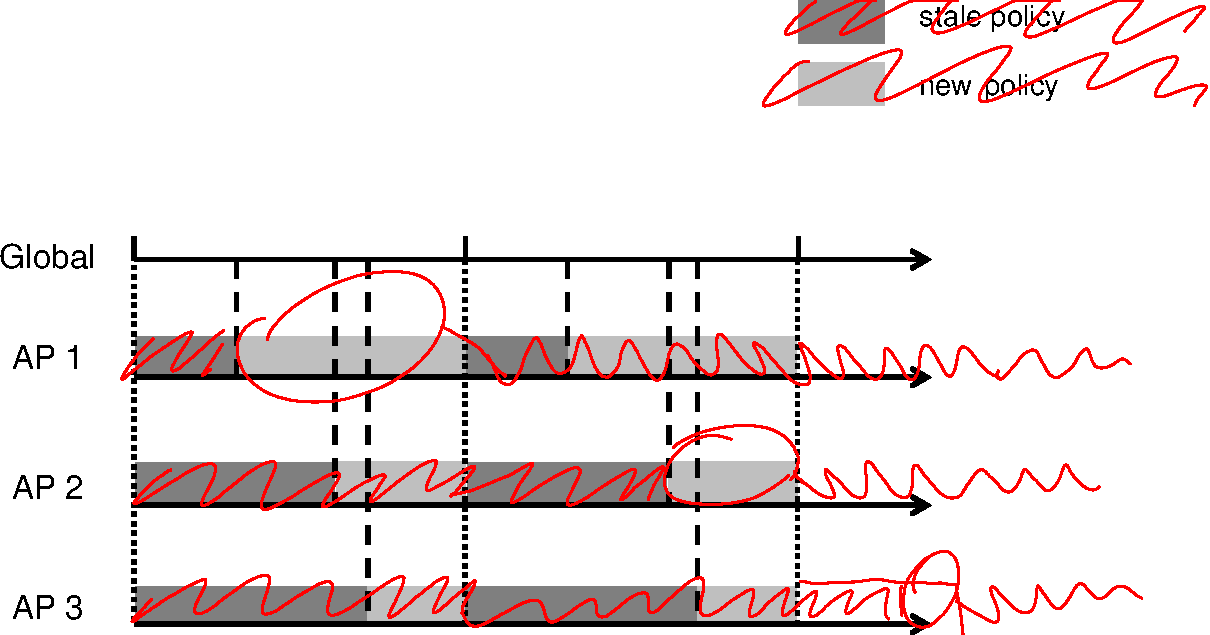
\includegraphics[width=0.45\textwidth]{brd-trans.pdf}
    \caption{Global System Transition with Partial Information-based Dispatching Decision}
    \label{fig:brd-trans}
\end{figure}

% NOTE: [partial and stale policy update definition]
% The \emph{dispatching policy} is applied over arrival jobs in each timeslot on each AP, and thus \emph{dispatching action space} is defined as $\mathbf{A}: (j, m) \in \jSpace \times \esSet$ where $(j, m)$ denotes the action that $j$-type job should be uploaded to $m$-th ES.
% \begin{definition}[Update Time Points]
%     For $k$-th AP ($\forall k\in\apSet$), partial updates firstly and then consensus update, which is defined as follows.
%     \begin{itemize}
%         \item Partial Update Point: The AP nodes will update their own policy when the corresponding \emph{Maximum Broadcast Latency} is achieved, and awareness of the previous policy change for the AP nodes receiving information before it;
%         \item Iterative Update Points: When reaching the ending of the broadcast interval, all the AP nodes would update the policy together;
%         this policy iteration is evaluated with no policy changes consideration in the following time in this interval;
%         this policy iteration is with partial information only with last interval, but not with information from this interval.
%     \end{itemize}
% \end{definition}
        
Based on the two stages of global broadcast information illustrated in system state, the compounded global-wise policy of all AP nodes is defined as follows.
\begin{definition}[Compounded Dispatching Policy]
    The compounded dispatching policy $\Policy(\Stat(t_{i}))$ over $\Stat(t_{i})$ which is defined with two-stage broadcasting information which is given as follows.
    \begin{align}
        \Policy(\Stat(t_{i})) \define \Bracket{
            \tilde{\Policy}(\Obsv(t_{i})), \tilde{\Policy}(\Obsv(t_{i-1}))
        },
    \end{align}
    where
    $\tilde{\Policy}(\Obsv(t_{i})) \define [\tilde{\Omega}_{1}(\Obsv(t_{i})), \dots, \tilde{\Omega}'_{K}(\Obsv(t_{i}))]$.
    The policy mapping over system state is further decoupled onto the two-stage broadcast information.

    Furthermore,
    $\tilde{\Omega}_{k}(\Obsv(t_{i}))$ in $\tilde{\Policy}(\Obsv(t_{i}))$
    denotes the local policy mapping over $\Obsv(t_{i})$ for $k$-th AP ($\forall k\in\apSet$), i.e. $k$-th AP would change its policy from $\tilde{\Omega}_{k}(\Obsv(t_{i-1}))$ to $\tilde{\Omega}_{k}(\Obsv(t_{i}))$ when receiving $\Obsv(t_{i})$.
    The explicit definition is given as follows.
    \begin{align}
        &\tilde{\Omega}_{k}(\Obsv(t_{i})) \define \set{\omega^{(k)}_{m,j}(t_{i})|\forall m\in\esSet, j\in\jSpace}
        ~(\forall k\in\apSet),
        \label{def_action}
    \end{align}
    where $\omega^{(k)}_{m,j}(t_{i})$ denotes the deterministic dispatching policy that: when $k$-th AP with information $\Obsv(t_{i})$, it would then upload $j$-type job to $m$-th ES if and only if $\omega^{(k)}_{m,j}(t_{i})=1$.
\end{definition}

We note that after the dispatching policy, the arrival distribution $A_{k,j}$ is further split onto different Edge Servers. The split arrival processes for $k$-th AP ($\forall k\in\apSet$) are still i.i.d Bernoulli distribution as
$\tilde{\lambda}^{(k)}_{m,j}(t_{i}) \define \lambda_{k,j} I[\omega^{(k)}_{m,j}(t_i) = 1]$ ($\forall m\in\esSet, j\in\jSpace$), where $I[\cdot]$ is indicator function.

%NOTE: [Multiple Phase of Iterative Update in Same Interval Example]
% More specifically, the multiple-phase of the policy $\tilde{\Omega}_k(\Obsv_i)$ at multiple \emph{iterative update points} are separated by \emph{Update Latency} $d_{k}(t_{i})$ for $k$-th AP ($k\in\apSet$). One vivid example of policy adaption phase is given as follows, the update rules of which will be elaborated in next sub-section.
% \begin{example}[Policy Phase Adaption]
%     In the time interval $[t_{i}, t_{i+1}]$, $k$-th AP would adopt $\tilde{\Omega}_{k}'(\Obsv_{i-1})$ immediately after $t_i$, and adopt $\tilde{\Omega}_{k}(\Obsv_{i})$ after its corresponding iterative update points; then with $\tilde{\Omega}_{k}'(\Obsv_{i})$ at $t_{i+1}$ and repeat the process.
% \end{example}
%----------------------------------------------------------------------------------------%

\subsection{The Optimization Problem}
We propose the jobs dispatching optimization problem with the target to minimize \emph{average response time} of all offloaded jobs in MEC system.
The \emph{average response time} is composed of uploading time from $AP$ to $ES$, and queueing-and-service time on corresponding ES. According to \emph{Little's Law}, the average response time of all jobs is equally as average number of jobs in system.
        
Due to the intrinsic property of periodic information broadcasting, we collect the cost for number counting at the pace of broadcasting interval which could be seems as sampling of original process based on timeslot scale.
Besides the cost counted for job response time, we furthermore add penalty on jobs submission over its capacity limit when the over-limited jobs will be rejected at the end of current broadcast interval.
Therefore, the cost function of this problem is given as follows.
\begin{align}
    g\Paren{\Stat(t_{i}), \Policy(\Stat(t_{i}))} \define&
    \sum_{k\in\apSet}\sum_{m\in\esSet}\sum_{j\in\jSpace} \Inorm{\vec{r}^{(k)}_{m,j}(t_{i})} + \sum_{m\in\esSet}\sum_{j\in\jSpace}
    \nonumber\\
    &\Brace{
        l_{m,j}(t_{i}) + \beta \mat{I}[l_{m,j}(t_{i})=L_Q]
    },
\end{align}
where $\Inorm{\vec{r}^{(k)}_{m,j}(t_i)}$ denotes the $L^1$-norm of vector $\vec{r}^{(k)}_{m}$, i.e. the sum up of absolute value of each entry; $\beta$ is weight factor for full-queue penalty.
        
Our distributed optimization problem definition is given as follows.
\begin{problem}[Original Cooperative Job Dispatching Problem]
    \begin{gather}
        \min_{\Policy} \lim_{T \to \infty}
            \mathbb{E}_{\Policy}
                \Bracket{\sum_{i=1}^{T} \gamma^{i-1} g\Paren{\Stat(t_{i}), \Policy(\Stat(t_{i}))}|\Stat(t_1)},
    \end{gather}
    where the cost is collected with a discount factor $\gamma$, \st{and $\Policy$ is optimized policy globally always with full-state information available.}
\end{problem}
According to \cite{sutton1998introduction}, the above problem could be solved by the following \emph{Bellman's equation}:
\begin{align}
    V(\Stat(t_i)) = &g(\Stat(t_i)) + \gamma \min_{\Policy(\Stat(t_{i}))}
        \nonumber\\
        & \sum_{\Stat(t_{i+1})} \Pr\{ \Stat(t_{i+1})|\Stat(t_{i}), \Policy(\Stat(t_{i})) \} \cdot V(\Stat(t_{i+1})).
    \label{sp_0}
\end{align}

However, the state information is actually partial-presence as $\Obsv(t_{i-1})$ at $t_i$ while $\Obsv(t_{i})$ would be available only after the random \emph{Update Latency} for each AP nodes.
This problem structure results into separated different acknowledge on when the policy should be updated for AP nodes. Thus we decouple the original problem into $K$-sub \hl{MDP-like problems} that update $\Policy$ in an iterative way which could at least converges to a sub-optimal solution.
        
For example, the $k$-th AP would update its policy in $k$-th sub-problem ($\forall k\in\apSet$) while the other AP nodes would keep with the previous policy. The corresponding Bellman's Equation is given as follows.
\begin{align}
    &V(\Stat(t_{i})) = g(\Stat_{i}) 
    \nonumber\\
    &~~~~+ \gamma \min_{\tilde{\Omega}_{k}(\Obsv(t_{i}))} \Pr\{ \Obsv(t_{i+1})|\Obsv(t_{i}), \Policy(\Stat(t_{i})) \} \cdot V(\Stat(t_{i+1})),
    \label{sp_k}
\end{align}
where $\tilde{\Omega}_{k}(\Obsv(t_{i}))$ is the component of $\Policy(\Obsv(t_{i}))$.
The performance improvement of next policy update is guaranteed by solution of Bellman's Equation with fixed policies from previous update.
The details and proof will be given in the following algorithm section.

% [abandon, Partial and iterative update points sub-problem definition]
% The first problem solves policy update at \emph{Partial Update Point} which assumes no policy update at \emph{Iterative Update Points}. The corresponding Bellman's Equation is defined as follows.
% \begin{align}
%     V(\Stat_{t_i}) = g(\Stat_{t_i}) + \gamma \min_{\Omega'(\Obsv_{i-1})} \Pr\{ \Obsv_{i+1}|\Obsv_{i-1}, \Policy(\Stat_{t_i}) \} V(\Stat_{i+1}),
%     \label{sp1}
% \end{align}
% where $\Policy(\Stat_{t_i}) = [\Omega'(\Obsv_{i-2}), \Omega(\Obsv_{i-1}), \Omega'(\Obsv_{i-1}), \Omega'(\Obsv_{i-1})]$ without policy update in $(t_i, t_{i+1}]$.      
% The second problem solves policy update at \emph{Iterative Update Points} which assumes no policy update at \emph{Partial Update Points}.
% Furthermore, the update is applied iteratively, as the name implies, with the order following length of broadcast latency (i.e. the sorted AP nodes order). The corresponding Bellman's Equation for $k$-th AP ($\forall k\in\apSet$) node is defined as follows.
% \begin{align}
%     V(\Stat_{t_i}) = g(\Stat_{t_i}) + \gamma \min_{\Omega^{(k)}(\Obsv_{i})} \Pr\{ \Obsv_{i+1}|\Obsv_{i}, \Policy(\Stat_{t_i}) \} V(\Stat_{i+1}),
%     \label{sp2}
% \end{align}
% where $\Omega^{(k)}(\Obsv_{i}) = [\tilde{\Omega}_{1}(\Obsv_{i}), \dots, \tilde{\Omega}_{k}(\Obsv_{i}), \tilde{\Omega}_{k+1}(\Obsv'_{i-1}), \dots, $ $\tilde{\Omega}_{K}(\Obsv'_{i-1})]$ in $\Policy(\Stat_{t_i})$.
% It implies that the updated policy before $k$-th AP must be known and thus impact the transition function of $k$-th AP.

To better analyze the optimization structure of the sub-problem, we decouple the transition function. The expression of transition function in Eqn. \ref{sp_k} is given as follows.
\begin{lemma}[Transition Function Decoupling]
    The transition function in Bellman's equation could be decoupled on AP nodes states and ES nodes states, which will facilitate the approximated value function expression in the following section.
    The decoupled transition function for Eqn. \ref{sp_k} is given as follows.
    \begin{align}
        & \Pr\{\Obsv(t_{i+1})|\Obsv(t_{i}), \Policy(\Stat(t_{i}))\}
        \nonumber\\
        =& \prod_{k\in\apSet}\prod_{m\in\esSet}\prod_{j\in\jSpace}
                \Pr\Brace{
                    \vec{r}^{(k)}_{m,j}(t_{i+1})|\vec{r}^{(k)}_{m,j}(t_{i}), \Policy(\Stat(t_{i}))
                }
                \times  
            \nonumber\\
            & \prod_{m\in\esSet}\prod_{j\in\jSpace}
                \Pr\Brace{
                    Q_{m,j}(t_{i+1})|Q_{m,j}(t_{i}), \mathcal{R}(t_{i}), \Policy(\Stat(t_{i}))
                }.
    \end{align}
\end{lemma}
\begin{proof}
    Proof deleted.
\end{proof}

The first part denotes the state transition on AP.
Denote as $\Pr\Brace{\vec{r}^{(k)}_{m,j}(t_{i+1})|\vec{r}^{(k)}_{m,j}(t_{i})} \sim \vecG{\Theta}^{(k)}_{m,j}(t_{i+1})$, where $\vecG{\Theta}^{(k)}_{m,j}(t_{i+1}) \define [\vecG{\theta}^{(k)}_{m,j,0}(t_{i+1}), \dots, \vecG{\theta}^{(k)}_{m,j,\Xi}(t_{i+1})]$.
Given that the uploading process could be depicted by the series of counters, we further have
$\Pr\Brace{r^{(k)}_{m,j,\xi+1}(t_{i+1})|r^{(k)}_{m,j,\xi}(t_{i})} \sim \vecG{\theta}^{(k)}_{m,j,\xi}(t_{i+1})$ ($\forall \xi=0,\dots,\Xi$).
Then we could express the distribution with a transition matrix as:
\begin{align}
    \vecG{\Theta}^{(k)}_{m,j}(t_{i+1}) \define \hat{\Gamma}^{(k)}_{m,j}\Paren{\Policy(\Stat(t_i)) }\vecG{\Theta}^{(k)}_{m,j}(t_{i}),
\end{align}
where transition matrix $\hat{\Gamma}^{(k)}_{m,j}$ is a \emph{block matrix}, whose element is transition matrix $\Gamma^{(k)}_{m,j,\xi}$ for the distribution on the series of counters. The definition is given as follows.
\begin{align}
    &\vecG{\theta}^{(k)}_{m,j,\xi+1}(t_{i+1}) \define
    \nonumber\\
    &\begin{cases}
        ( \Gamma^{(k)}_{m,j,\xi} \dots \Gamma^{(k)}_{m,j,\xi-N} ) \times \vecG{\theta}^{(k)}_{m,j,\xi-N-1}(t_i), &{\xi \geq N}
        \\
        ( \Gamma^{(k)}_{m,j,\xi} \dots \Gamma^{(k)}_{m,j,1} ) \times \vecG{\theta}^{(k)}_{m,j,0}(t_i), &{\xi < N}
    \end{cases},
\end{align}
where $\vecG{\theta}^{(k)}_{m,j,0}(t_{i}) \sim \text{Bernoulli}(\tilde{\lambda}^{(k)}_{m,j}(t_i))$, and transition matrix $\Gamma^{(k)}_{m,j,\xi}$ is time-invariant and defined as follows.
\begin{align}
    \Gamma^{(k)}_{m,j,\xi} = 
    \begin{bmatrix}
        &0 \\
        &p^{(k)}_{m,j,\xi} &\bar{p}^{(k)}_{m,j,\xi} \\
        &(p^{(k)}_{m,j,\xi})^2 &2(p^{(k)}_{m,j,\xi}\bar{p}^{(k)}_{m,j,\xi}) &(\bar{p}^{(k)}_{m,j,\xi})^2 \\
        % &(p^{(k)}_{m,j,\xi})^3 &3(p^{(k)}_{m,j,\xi})^2(\bar{p}^{(k)}_{m,j,\xi}) &3(p^{(k)}_{m,j,\xi})(\bar{p}^{(k)}_{m,j,\xi})^2 &(p^{(k)}_{m,j,\xi})^3 \\
        &\dots &\dots &\dots &\dots
    \end{bmatrix}^T,
\end{align}
where $p^{(k)}_{m,j,\xi} \define \Pr\{U^{(k)}_{m,j} < (\xi+1) | U^{(k)}_{m,j}>\xi\}$ and $\bar{p}^{(k)}_{m,j,\xi} = 1 - p^{(k)}_{m,j,\xi}$.
And $\hat{\Gamma}^{(k)}_{m,j}$ is an off-diagonal block matrix plus the horizontal part w.r.t $\vecG{\theta}^{(k)}_{m,j,0}$, with other entries as zero.

The second part denotes the state transition on ES.
Denote $\Pr\Brace{ Q_{m,j}(t_{i+1})|Q_{m,j}(t_{i}), \mathcal{R}(t_{i}) } \sim \vecG{\nu}_{m,j}(t_i)$. We notice that the job arrival distribution $\vecG{\beta}_{m,j}(t_{i})$ is given by $\mathcal{R}(t_{i})$, and the departure rate in one slot is deterministic as $1/N$.
Thus the expectation of $\vecG{\beta}$ would be always far more smaller than $1$ as composed all all $K$ AP nodes.
We take approximation on $\vec{\beta}$ as Bernoulli distribution in each time slot that $\vecG{\beta}(t_{i,n}) \triangleq [\beta^{(0)}_{m,j}(t_{i,n}), \beta^{(1)}_{m,j}(t_{i,n})]$, where
\begin{align}
    \beta^{(1)}_{m,j}(t_{i,n}) &\define \sum_{k\in\mathcal{K}} \sum_{\xi=0,\dots,\Xi-1} \mathbb{E}[\vecG{\rho}^{(k,+)}_{m,j,\xi}(t_{i,n})]
    \label{eqn_0}
    \\
    \vecG{\rho}^{(k,+)}_{m,j,\xi}(t_{i,n}) &\define \tilde{\Gamma}^{(k)}_{m,j,\xi} \times \vecG{\theta}^{(k)}_{m,j,\xi}(t_{i,n})
    % \label{eqn_1}
    \\
    \beta^{(0)}_{m,j}(t_{i,n}) &= 1-\beta^{(1)}_{m,j}(t_{i,n})
    % \label{eqn_2}
\end{align}
And we could obtain the time-variant transition matrix composed of multiple transition matrix $P_{m,j}(\vecG{\beta}(t_{i,n}))$ in all the time slots in $i$-th interval as follows.
\begin{align}
    \vecG{\nu}(t_{i,n+1}) &= P_{m,j}\Paren{\vecG{\beta}(t_{i,n})} \vecG{\nu}(t_{i,n})
    % \label{eqn_3}
    \\
    \vecG{\nu}(t_{i+1}) &= \prod_{n=0,\dots,N-1} P_{m,j}\Paren{\vecG{\beta}(t_{i,n})} \vecG{\nu}(t_{i}),
    \label{eqn_4}
\end{align}
%FIXME: could/should we give explicit definition for $P_{m,j}$ ?
% where
% \begin{align}
%     \Paren{ P_{m,j}(\vecG{\beta}(t_{i,n})) }_{} \define 
%     \begin{cases}
%         , &\eta_{m,j} = 1
%         \\
%         , &\eta_{m,j} > 1
%     \end{cases}
% \end{align}

However, after the state decomposition, the action space would still be exponentially expanded with respect to number AP and ES nodes. We could not use traditional \emph{policy iteration} or \emph{value iteration} algorithm \cite{sutton1998introduction} for unacceptable computational complexity.
So in next section, to alleviate curse of dimensionality, we introduce baseline dispatching policy to approximate the value function, and then carry out one-step iteration to obtain a better value function approximation.
%----------------------------------------------------------------------------------------%